%%=============================================================================
%% Methodologie
%%=============================================================================

\chapter{\IfLanguageName{dutch}{Methodologie}{Methodology}}
\label{ch:methodologie}

In de stand van zaken werden de verschillende te vergelijken module bundlers toegelicht. Deze zullen in dit hoofdstuk naast elkaar gelegd en gequoteerd aan de hand van verscheidene factoren. 
Eerst zal gekeken worden hoe ze verschillen bij het opzetten van een nieuw project. Daarna trachten we een bestaand project dat met Webpack opgezet is, om te vormen naar een van de andere opties. In het volgend hoofdstuk volgt de conclusie.

Eerst en vooral is er nood aan bestaande projecten om de build tools te kunnen testen. Gelukkig zijn er online genoeg open-source voorbeelden hiervan te vinden. Drie projecten werden gekozen aan de hand van hun grootte en technologieën die ze gebruiken. Eén eigenschap hebben ze allemaal gemeen: het zijn Javascript projecten die React als UI library gebruiken. De reden dat geen projecten gekozen zijn die andere UI libraries zoals Vue gebruiken, is omdat React veel meer gebruikt wordt, ook door de co-promotor. Desondanks zijn de gekozen projecten ook representatief voor de andere UI libraries omdat ze uiteindelijk allemaal Javascript zijn. 

Volgende factoren worden gebruikt om een eenduidige vergelijking te maken. Daarnaast zullen meer subjectieve factoren, gelijk de gemakkelijkheid om het werkende te krijgen, aan bod komen.
\begin{itemize}
    \item Output bundle grootte
    \item Output bundle snelheid
    \item Snelheid bij wijziging
    \item Opstartsnelheid development server
\end{itemize}

\section{Nieuw project}
\subsection{Webpack}
Een nieuw project opzetten met Webpack kan op verschillende manieren: zelf een project opzetten en de configuratie volledig manueel schrijven of gebruik maken van een framework waarin het al geconfigureerd voor ons is. Aangezien niet velen het eerste pad bewandelen, zullen we gebruik maken van de meest populaire manier om een React project op te zetten. Create-react-app of CRA is een minimale framework gemaakt door de makers van React zelf om gemakkelijk een React omgeving op te zetten. Het is één van de vele frameworks die Webpack als module bundler gebruikt. Om te beginnen, voeren we volgende commando’s uit. 

\lstinputlisting[language=bash]{codeSnippets/craCreate.txt}

Bovenstaande code maakt een project aan met create-react-app. Daarna ziet ons project er als volgt uit. Merk op dat er geen config bestand voor Webpack is.

\begin{figure}[h]
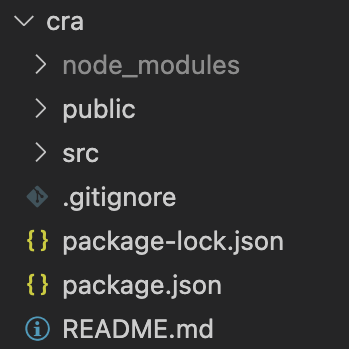
\includegraphics{fileStructureInitCRA}
    \centering
    \caption[]{Bestandsstructuur nieuw CRA project}
\end{figure}

Alles wat in de public map staat, zijn statische assets. Die zullen dus via een url bereikbaar zijn. Als we kijken in het index.html bestand, merken we op dat er geen enkele script-tag aanwezig is. Hierover later meer.
In de src map staat alles wat door Webpack zal gebundeld worden. Standaard worden er CSS bestanden aangemaakt voor styling en een logo in svg formaat. Dit wordt gedaan om aan te tonen dat we deze assets gewoon in de Javascript code kunnen importeren, de bundler kan hiermee overweg. 

\lstinputlisting[language=Javascript]{codeSnippets/importCSS.js}

In het package.json bestand staat er allemaal info over dit project. In het dependencies gedeelte staan alle externe packages die dit project gebruikt. Nieuwe packages worden gedownload aan de hand van Node Package Manager of NPM. Bij de dependencies staat een package genaamd “react-scripts”. 
React-scripts \autocite{facebook-2018} is een package gemaakt door de makers van React en is de motor achter CRA. 
Wat voor dit onderzoek relevant is, is dat het de Webpack.config bevat. Dit bestand bestaat uit maar liefst 700+ lijnen code \autocite{facebook-2021}. Nu is de reden dat we CRA gebruiken en niet van nul beginnen, duidelijk. 

De volgende stap is om het project lokaal op te starten. React-scripts gebruikt de ingebouwde development server van Webpack. Na het uitvoeren van volgend commando, wordt die server opgestart en opent de webapplicatie in een browser.

\lstinputlisting[language=bash]{codeSnippets/craStart.txt}

\begin{table}[h]
    \centering
    \begin{tabular}{lr}
    \textbf{Grootte project (MB)} & 0,037 \\
    \textbf{Grootte node\_modules (MB)} & 214,1 \\
    \textbf{Grootte uitvoer (MB)} & 0,514 \\
    \textbf{Snelheid creatie uitvoer (s)} & 3,67 \\
    \textbf{} & 5 \\
    \textbf{} & 3 \\
    \textbf{} & 3 \\
    \textbf{Snelheid opstarten development server (s)} & 2,67 \\
    \textbf{} & 4 \\
    \textbf{} & 2 \\
    \textbf{} & 2
    \end{tabular}
    \caption[]{Overzicht nieuw project met Webpack}
    \end{table}

\subsection{Parcel}
Bij Webpack gebruikten we een framework om het vele configuratie werk te omzeilen. Bij Parcel is dit niet nodig. Zoals in de literatuurstudie vermeld werkt Parcel op een gelijkaardige manier als Webpack, maar dan met zo min mogelijk configuratie. Om een nieuw project op te zetten, gaan we dus geen framework gebruiken.

Maak een nieuwe map aan waar het project zal leven. Aangezien we van nul beginnen, moeten de bestanden uit figuur 3.2 zelf aangemaakt worden.

\begin{figure}[h]
    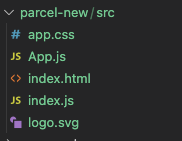
\includegraphics{parcelNew}
        \centering
        \caption[]{Aan te maken bestanden voor nieuw Parcel project}
    \end{figure}

    Hierna moeten er nog enkele packages geïnstalleerd worden, namelijk: React, React-DOM en natuurlijk Parcel. In de package.json moet er ook nog meegegeven worden waar de index.html zich bevindt. Merk op dat er geen apart configuratiebestand voor Parcel is. Nu kan het project opgestart worden met hetzelfde commando als bij Webpack.

    Merk op dat er geen public folder aanwezig is zoals in CRA. Er is momenteel geen folder waar statische bestanden kunnen leven. Als dit een vereiste is, heeft Parcel een plugin nodig. Gelukkig zijn die gemakkelijk te installeren.

\subsection{Snowpack}
Voor Snowpack gaan we net zoals bij Parcel te werk zonder framework. In tegenstelling tot Parcel heeft het Snowpack team al een speciaal react-template gemaakt met een kant en klaar commando om het te initialiseren. Zelf de bestanden aanmaken en dependencies toevoegen is dus niet nodig.

\lstinputlisting[language=bash]{codeSnippets/snowpackNew.txt}
\begin{figure}[h]
    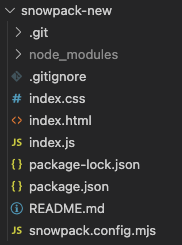
\includegraphics{snowpackNew}
        \centering
        \caption[Aangemaakte bestanden door Snowpack commando]{Aangemaakte bestanden door commado}
    \end{figure}

Deze structuur is identiek aan die van CRA. In tegenstelling tot Parcel is een public folder al geconfigureerd waar statische bestanden, zoals afbeeldingen, beschikbaar staan. Een configuratiebestand voor Snowpack is ook aangemaakt. Hierin staan al 25 lijnen configuratie voor ons geschreven. Meer dan Parcel maar aanzienlijk minder dan CRA. Merk op dat sommige bestanden nu de extensie .jsx in plaats van .js hebben. Dit komt doordat Snowpack geen JSX tolereert in .js bestanden. JSX is wat een React component retourneert i.e elk React component moet een .jsx extensie hebben. Geen probleem bij een nieuw project maar bij een oud kan het nodig zijn om vele bestanden van extensie te veranderen, zie later.

Zoals in de literatuurstudie vermeld, is Snowpack geen module bundler aangezien het de verschillende bestanden in een project niet bundelt. In productie kan dat optioneel nog gedaan worden door Webpack of Rollup maar dat is niet standaard. In development heeft dit het grote voordeel dat de bundel niet telkens opnieuw opgebouwd moet worden als een bestand veranderd. 

\subsection{Vite}
Vite is nog een voorbeeld van een unbundled build tool, net zoals Snowpack. Een nieuw project opzetten is heel gemakkelijk aan de hand van een simpel commando dat ze voorzien hebben, net zoals Snowpack. 

\lstinputlisting[language=bash]{codeSnippets/viteNew.txt}

\begin{figure}[h]
    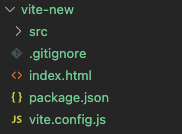
\includegraphics{viteNew}
        \centering
        \caption[Aangemaakte bestanden door Vite commando]{Aangemaakte bestanden door commado}
    \end{figure}

Er is een klein config bestand aanwezig van 7 lijnen code waar de react plugin is geïnitialiseerd. Voor de rest ziet het project in grote lijnen er uit als dat van Snowpack. Er is geen public map aanwezig maar dat kan aangemaakt worden en wordt automatisch geconfigureerd.

\section{Bestaand project}
In het vorige deel, werden nieuwe projecten opgezet voor de respectievelijke module bundlers. In dit deel worden bestaande projecten, opgezet met Webpack, omgevormd zodat ze gebruik maken van de andere opties. Per project wordt eerst wat toelichting gegeven en vervolgens per module bundler wat er nodig is om ze werkende te krijgen. 

\subsection{Mortage}
Mortage \autocite{houghton-2019}

\subsubsection{Parcel}
Zoals in de literatuurstudie vermeld, probeert Parcel hetzelfde als Webpack te bereiken maar met veel minder tot geen configuratie. Die claim zullen we nu op de som nemen. Mortage is opgezet met CRA en gebruikt dus het react-scripts package die onder andere alle Webpack config op zich neemt. Om Webpack in te ruilen voor Parcel moeten we dus eerst react-scripts bij het grofvuil zetten. Het package.json bestand bevat alle info over een project: de naam, versie, welke andere packages het gebruikt, hoe het wordt opgestart en nog veel meer. Ook Mortage heeft zo’n bestand en dat ziet er als volgt uit:


In het gedeelte “scripts” staan de custom scripts voor ons project. Het start en build commando starten het project in development en production mode respectievelijk. Beide voeren zij op hun beurt een commando van react-scripts uit. Dit gaat dus vervangen moeten worden. In de documentatie van Parcel valt te lezen dat we die commando’s moeten vervangen met de volgende:

Vervolgens moet het index.html bestand aangepast worden. Voor de wijzigingen zag het er als volgt uit:

Merk op dat er nergens een verwijzing is naar een Javascript bestand. React-scripts voegt dat automatisch toe bij het bouwen van het project. Parcel doet dat niet dus er moet nog een expliciete verwijzing komen. Nadien ziet het bestand er als volgt uit:

Nu moet Parcel uiteraard nog gedownload worden. Nadien werkt het project. Op het einde van deze sectie staan alle vergelijkende data.

\subsubsection{Snowpack}
Snowpack gebruikt de principes van unbundled development uitgelegd in de literatuurstudie. Wat dat betekent in de werkelijkheid volgt later. Eerst kijken we hoe Mortage kan omgevormd worden van Webpack naar Snowpack. 

Bij Parcel lag de focus op zo weinig mogelijk configuratie, niet bij Snowpack. Snowpack is veel moeilijker te configureren dan Parcel en Vite en voelt in dat opzicht aan als Webpack. We ondernemen dezelfde stappen als hierboven om react-scripts te verwijderen en die te vervangen door de nieuwe commando’s. Daarna voegen we Snowpack toe samen met twee andere plugins voor React. We doen net dezelfde wijzigingen aan index.html, voegen een configuratie bestand toe en proberen de app te runnen. Een foutmelding verschijnt, om die te kunnen begrijpen, is er eerst wat meer uitleg nodig.

Een React component retourneert JSX. JSX is, zonder te veel in details te gaan, een extensie bovenop Javascript die een manier biedt om de weergave van componenten te structureren en lijkt heel hard op HTML. Het belangrijke om hiervan mee te nemen is dat het een Javascript extensie is. In CRA en sommige andere frameworks is het mogelijk om JSX in een bestand te schrijven met de standaard Javascript extensie .js . Snowpack ondersteunt dit niet. Als er een bestand JSX bevat, moet die de extensie .jsx hebben. Dus moeten we alle bestanden die JSX gebruiken van bestandsextensie veranderen. Hierna werkt de app naar behoren. 

\subsubsection{Vite}
Vite combineert het beste van de twee voorgaande build tools. Het gebruikt de principes van unbundled development en dat met weinig configuratie. Om Mortage op te zetten met Vite overlopen we stappen die eerder al aan bod kwamen: react-scripts verwijderen, index.html en package.json naar de nieuwe commando’s aanpassen en Vite zelf installeren. Net zoals Snowpack ondersteunt Vite geen JSX in een .js bestand en is er een plugin voor React. In tegenstelling tot Snowpack is de plugin niet nodig om het project werkend te krijgen. Na dit alles kan het project zonder problemen opgestart worden. 

\subsection{Mortage}

\subsubsection{Parcel}
Om dit project om te vormen naar Webpack overlopen worden eerst dezelfde stappen doorlopen als in het vorig. Er zijn twee mogelijke extra struikelblokken voor Todoist: het gebruik van SCSS en statische bestanden. Het eerste overkomt Parcel met glans: we moeten niets zelf configureren. De eerste keer dat Todoist wordt gestart, detecteert Parcel dat er SCCS aanwezig is en download de bijhorende plugin hiervoor. Het tweede probleem vereist ook een plugin en daarenboven nog wat configuratie. In de package.json duiden we met volgende lijnen aan waar het mapje met statische bestanden zich bevindt. Nadien moeten de links naar de afbeeldingen nog veranderd worden naar de nieuwe locatie. Hierna is ook dit project bijna klaar voor gebruik. Enkel nog het configuratie bestand voor de database moet nog aangepast worden.

\subsubsection{Snowpack}
Ook hier zijn de stappen gelijkaardig aan het vorig project. Na die te doorlopen volgen nog twee potentiële moeilijkheden. In het vorig deel over Snowpack werd al vermeld dat statistische bestanden ondersteunt worden zonder extra plugin. Het tweede probleem, SCSS, kan eveneens opgelost worden door een plugin. In tegenstelling tot Parcel, moet die wel manueel toegevoegd worden. 

\subsubsection{Vite}
Voor Vite kunnen we heel kort blijven. Na het uitvoeren van dezelfde stappen als vorig project, werkt alles. Zowel statische bestanden als SCCS zijn ondersteunt zonder extra plugins of configuratie.

\subsection{Bar}

\subsubsection{Parcel}

\subsubsection{Snowpack}


\subsubsection{Vite}
Na de hele waslijst problemen die bij Snowpack opdoken, doet het deugd om weer met Vite aan de slag te mogen. Van de struikelblokken die Snowpack tegenkwam, blijft voor Vite enkel nog het probleem van de CommonJS module over. Na die te herschrijven en dezelfde stappen te doorlopen als bij de vorige Vite secties, werkt dit project volledig, ook Workbox. Typescript wordt ook ondersteunt zonder extra gedoe en voor Tailwind is de gebruikelijke installatie en configuratie nodig, geen extra plugin nodig. Net zoals bij Parcel moeten de verwijzingen naar de afbeeldingen in de index.html bijgeschaafd worden. 


De conclusie over de bevindingen die in dit hoofdstuk waargenomen zijn, volgt in het volgend hoofdstuk. 

